%                                                                 aa.dem
% AA vers. 9.1, LaTeX class for Astronomy & Astrophysics
% demonstration file
%                                                       (c) EDP Sciences
%-----------------------------------------------------------------------
%
% \documentclass[referee]{aa} % for a referee version
%\documentclass[onecolumn]{aa} % for a paper on 1 column  
%\documentclass[longauth]{aa} % for the long lists of affiliations 
%\documentclass[letter]{aa} % for the letters 
%\documentclass[bibyear]{aa} % if the references are not structured 
%                              according to the author-year natbib style

%

\documentclass{aa}  

%
\usepackage{graphicx}
\usepackage{amsmath,amsfonts,amssymb}
\usepackage{natbib}


%%%%%%%%%%%%%%%%%%%%%%%%%%%%%%%%%%%%%%%%
\usepackage{txfonts}
\usepackage{xcolor}

\usepackage{blindtext}
%%%%%%%%%%%%%%%%%%%%%%%%%%%%%%%%%%%%%%%%
% \usepackage[options]{hyperref}
% To add links in your PDF file, use the package "hyperref"
% with options according to your LaTeX or PDFLaTeX drivers.
\usepackage{float}
%\usepackage{stfloats}
\usepackage{dblfloatfix}
\usepackage{afterpage}
\usepackage{ifthen}
\usepackage[morefloats=12]{morefloats}

\usepackage{placeins}
\usepackage{multicol}
\usepackage[export]{adjustbox}\usepackage[breaklinks,colorlinks,citecolor=blue]{hyperref}
\bibpunct{(}{)}{;}{a}{}{,}
\usepackage[switch]{lineno}
\definecolor{linkcolor}{rgb}{0.6,0,0}
\definecolor{citecolor}{rgb}{0,0,0.75}
\definecolor{urlcolor}{rgb}{0.12,0.46,0.7}
%\usepackage[breaklinks, colorlinks, urlcolor=urlcolor,linkcolor=linkcolor,citecolor=citecolor,pdfencoding=auto]{hyperref}
\hypersetup{linktocpage}
\usepackage{bold-extra}
\usepackage{tabularx, booktabs}

%Planck style file, to be used with A&A style to produce Planck papers for publication.
%
% version 28 September 2010 --- useful macros --- CRL
% version 17 October 2010   --- first cut at important instrument values, from Daniele Mennella and
%                               Francois Bouchet, 13 October 2010 --- CRL
% version 18 October 2010   --- LFI FWHM changed to one value per feed, rather than M & S separately
%                               LFI FWHM uncertainties added for individual feeds.  Corrections made
%                               to LFI values. --- Andrea Zacchei
% version 24 October 2010   --- added to and corrected definitions.  No changes made to instrument
%                               quantities. --- CRL 
% version 31 October 2010   --- added definition of \muKHz. --- CRL
%
% version 15 November 2010  --- fixed conflict with aa.cls in definition of \endtable
%                               by naming the command below "\endPlancktable".  See section
%                               13.16 of the Style Guide.
%
% version 06 December 2010  --- Set up names with and without units.
%                               Add \allearlypapers command to ensure that all early papers are
%                               included in the reference list.
%                               Define macro for the name of the 4He JT cooler.
%
% version 07 December 2010  --- removed extraneous "planck2011-1.2" entry in \allearlypapers
%
% version 12 December 2010  --- added \endPlancktablewide command to set tablenotes to the full
%                               page width in the \begin{table*}...\end{table*} environment when
%                               the ``twocolumn'' option is specified in the \documentclass command.
%                               (It would be more elegant to extract the appropriate width from the
%                               aa.cls system at the time of execution, but that is buried more
%                               deeply in the system than I investigated.)
%
% version 05 January 2011   --- added unit \MJysr.  HFI performance values updated per FRB email
%                               01/05/2011 02:38-0800, and Brendan Crill email 01/05/2011 18:08 -0800.
%
% version 06 January 2011   --- changed \scriptscriptstyle primes to \scriptstyle, to better match the
%                               tx fonts used by A&A.
%
% version 07 January 2011   --- modified \allearlypapers to correspond with final early paper list.  
%                               Fixed 545 GHz center frequency.
%
% version 07 January 2011b  --- changed LFI white-noise sensitivity numbers to correct problem with units
%
% version 05 July 2011      --- added \Msol and \Lsol to get the symbols for solar mass and luminosity.
%                               Deleted previous definitions of \solar and \sol, which were equivalent
%                               to the new \Msol.
%
% version 16 August 2011    --- changed comments on \endPlancktable and \endPlancktablewide for clarity
%
% version 11 September 2011 --- changed definition of \tablenote to make footnote labels italic, as per A\&A
%
% version 26 April 2011     --- changed definition of \Planck to agree with what is said in the Style Guide (!)
%
% version 04 Dec 2013       --- included 2013 results references
%
% version 17 Jan 2014       --- included fix to bibtex file v4.3, i.e. \providecommand{\sorthelp}[1]{}
%
% version 26 Jul 2014       --- fixed incompatibility problem with aa.cls v8.0 and v8.2.  v8.2 should now be used
%                               for all Planck papers.
%                           --- fixed problem in definition of "\all2013resultspapers" that introduced a blanck
%                               into the reference to p06b.
%                           --- removed all the parameter definition stuff at the end.  We weren't using it, and
%                               it took up a lot of space.
%
% version 28 Jan 2015       --- added "\alltwentyfiftennresultspapers" and corrected "\all2013resultspapers" to
%                               "\all20thirteenresultspapers",
%
% Usage:  after the \documentclass[traditabstract]{aa} command in the La\TeX\ input file,
%         add this command:      \input Planck.tex


\def\setsymbol#1#2{\expandafter\def\csname #1\endcsname{#2}}
\def\getsymbol#1{\csname #1\endcsname}

%-----------------------------------------------------------------------
% Planck
%-----------------------------------------------------------------------
\def\Planck{\textit{Planck}}

%-----------------------------------------------------------------------
% The Planck Helium-4 JT cooler
%-----------------------------------------------------------------------
\def\HeJT{$^4$He-JT}

%-----------------------------------------------------------------------
% To include all Planck Early Results papers in the reference lists
%-----------------------------------------------------------------------
\def\allearlypapers{\nocite{planck2011-1.1, planck2011-1.3, planck2011-1.4, planck2011-1.5, planck2011-1.6, planck2011-1.7, planck2011-1.10, planck2011-1.10sup, planck2011-5.1a, planck2011-5.1b, planck2011-5.2a, planck2011-5.2b, planck2011-5.2c, planck2011-6.1, planck2011-6.2, planck2011-6.3a, planck2011-6.4a, planck2011-6.4b, planck2011-6.6, planck2011-7.0, planck2011-7.2, planck2011-7.3, planck2011-7.7a, planck2011-7.7b, planck2011-7.12, planck2011-7.13}}

%-----------------------------------------------------------------------
% To include all Planck 2013 Results papers in the reference lists
%-----------------------------------------------------------------------
\def\alltwentythirteenresultspapers{\nocite{planck2013-p01, planck2013-p02, planck2013-p02a, planck2013-p02d, planck2013-p02b, planck2013-p03, planck2013-p03c, planck2013-p03f, planck2013-p03d, planck2013-p03e, planck2013-p01a, planck2013-p06, planck2013-p03a, planck2013-pip88, planck2013-p08, planck2013-p11, planck2013-p12, planck2013-p13, planck2013-p14, planck2013-p15, planck2013-p05b, planck2013-p17, planck2013-p09, planck2013-p09a, planck2013-p20, planck2013-p19, planck2013-pipaberration, planck2013-p05, planck2013-p05a, planck2013-pip56, planck2013-p06b, planck2013-p01a}}

%-----------------------------------------------------------------------
% To include all Planck 2015 Results papers in the reference lists
%-----------------------------------------------------------------------
\def\alltwentyfifteenresultspapers{\nocite{planck2014-a01, planck2014-a03, planck2014-a04, planck2014-a05, planck2014-a06, planck2014-a07, planck2014-a08, planck2014-a09, planck2014-a11, planck2014-a12, planck2014-a13, planck2014-a14, planck2014-a15, planck2014-a16, planck2014-a17, planck2014-a18, planck2014-a19, planck2014-a20, planck2014-a22, planck2014-a24, planck2014-a26, planck2014-a28, planck2014-a29, planck2014-a30, planck2014-a31, planck2014-a35, planck2014-a36, planck2014-a37, planck2014-ES}}

%-----------------------------------------------------------------------
% Tables
%-----------------------------------------------------------------------
\newbox\tablebox    \newdimen\tablewidth
\def\leaderfil{\leaders\hbox to 5pt{\hss.\hss}\hfil}
%
% use the following definition of \endPlancktable for ApJ style notes to tables, set to the 
%         width of the table
% \def\endPlancktable{\tablewidth=\wd\tablebox 
%
% use the following definitions of \endPlancktable and \endPlancktablewide for A&A style notes 
% set to one-column  or full-page width, respectively
\def\endPlancktable{\tablewidth=\columnwidth 
    $$\hss\copy\tablebox\hss$$
    \vskip-\lastskip\vskip -2pt}
\def\endPlancktablewide{\tablewidth=\textwidth 
    $$\hss\copy\tablebox\hss$$
    \vskip-\lastskip\vskip -2pt}
\def\tablenote#1 #2\par{\begingroup \parindent=0.8em
    \abovedisplayshortskip=0pt\belowdisplayshortskip=0pt
    \noindent
    $$\hss\vbox{\hsize\tablewidth \hangindent=\parindent \hangafter=1 \noindent
    \hbox to \parindent{$^#1$\hss}\strut#2\strut\par}\hss$$
    \endgroup}
\def\doubleline{\vskip 3pt\hrule \vskip 1.5pt \hrule \vskip 5pt}

%-----------------------------------------------------------------------
% useful macros
%-----------------------------------------------------------------------
%
\def\L2{\ifmmode L_2\else $L_2$\fi}
%
\def\dtt{\Delta T/T}
\def\DeltaT{\ifmmode \Delta T\else $\Delta T$\fi}
\def\deltat{\ifmmode \Delta t\else $\Delta t$\fi}
\def\fknee{\ifmmode f_{\rm knee}\else $f_{\rm knee}$\fi}
\def\Fmax{\ifmmode F_{\rm max}\else $F_{\rm max}$\fi}
%
\def\solar{\ifmmode{\rm M}_{\mathord\odot}\else${\rm M}_{\mathord\odot}$\fi}
\def\Msolar{\ifmmode{\rm M}_{\mathord\odot}\else${\rm M}_{\mathord\odot}$\fi}
\def\Lsolar{\ifmmode{\rm L}_{\mathord\odot}\else${\rm L}_{\mathord\odot}$\fi}
%
\def\inv{\ifmmode^{-1}\else$^{-1}$\fi}
\def\mo{\ifmmode^{-1}\else$^{-1}$\fi}
\def\sup#1{\ifmmode ^{\rm #1}\else $^{\rm #1}$\fi}
\def\expo#1{\ifmmode \times 10^{#1}\else $\times 10^{#1}$\fi}
%
\def\,{\thinspace}
\def\lsim{\mathrel{\raise .4ex\hbox{\rlap{$<$}\lower 1.2ex\hbox{$\sim$}}}}
\def\gsim{\mathrel{\raise .4ex\hbox{\rlap{$>$}\lower 1.2ex\hbox{$\sim$}}}}
\let\lea=\lsim
\let\gea=\gsim
\def\simprop{\mathrel{\raise .4ex\hbox{\rlap{$\propto$}\lower 1.2ex\hbox{$\sim$}}}}
%
\def\deg{\ifmmode^\circ\else$^\circ$\fi}
\def\pdeg{\ifmmode $\setbox0=\hbox{$^{\circ}$}\rlap{\hskip.11\wd0 .}$^{\circ}
          \else \setbox0=\hbox{$^{\circ}$}\rlap{\hskip.11\wd0 .}$^{\circ}$\fi}
\def\arcs{\ifmmode {^{\scriptstyle\prime\prime}}
          \else $^{\scriptstyle\prime\prime}$\fi}
\def\arcm{\ifmmode {^{\scriptstyle\prime}}
          \else $^{\scriptstyle\prime}$\fi}
\newdimen\sa  \newdimen\sb
\def\parcs{\sa=.07em \sb=.03em
     \ifmmode \hbox{\rlap{.}}^{\scriptstyle\prime\kern -\sb\prime}\hbox{\kern -\sa}
     \else \rlap{.}$^{\scriptstyle\prime\kern -\sb\prime}$\kern -\sa\fi}
\def\parcm{\sa=.08em \sb=.03em
     \ifmmode \hbox{\rlap{.}\kern\sa}^{\scriptstyle\prime}\hbox{\kern-\sb}
     \else \rlap{.}\kern\sa$^{\scriptstyle\prime}$\kern-\sb\fi}
%
\def\ra[#1 #2 #3.#4]{#1\sup{h}#2\sup{m}#3\sup{s}\llap.#4}
\def\dec[#1 #2 #3.#4]{#1\deg#2\arcm#3\arcs\llap.#4}
\def\deco[#1 #2 #3]{#1\deg#2\arcm#3\arcs}
\def\rra[#1 #2]{#1\sup{h}#2\sup{m}}
%
\def\page{\vfill\eject}
\def\dots{\relax\ifmmode \ldots\else $\ldots$\fi}
%
%-----------------------------------------------------------------------
% units
%-----------------------------------------------------------------------
%
\def\WHzsr{\ifmmode $W\,Hz\mo\,sr\mo$\else W\,Hz\mo\,sr\mo\fi}
\def\mHz{\ifmmode $\,mHz$\else \,mHz\fi}
\def\GHz{\ifmmode $\,GHz$\else \,GHz\fi}
\def\mKs{\ifmmode $\,mK\,s$^{1/2}\else \,mK\,s$^{1/2}$\fi}
\def\muKs{\ifmmode \,\mu$K\,s$^{1/2}\else \,$\mu$K\,s$^{1/2}$\fi}
\def\muKRJs{\ifmmode \,\mu$K$_{\rm RJ}$\,s$^{1/2}\else \,$\mu$K$_{\rm RJ}$\,s$^{1/2}$\fi}
\def\muKHz{\ifmmode \,\mu$K\,Hz$^{-1/2}\else \,$\mu$K\,Hz$^{-1/2}$\fi}
\def\MJysr{\ifmmode \,$MJy\,sr\mo$\else \,MJy\,sr\mo\fi}
\def\MJysrmK{\ifmmode \,$MJy\,sr\mo$\,mK$_{\rm CMB}\mo\else \,MJy\,sr\mo\,mK$_{\rm CMB}\mo$\fi}
\def\microns{\ifmmode \,\mu$m$\else \,$\mu$m\fi}
\def\micron{\microns}
\def\muK{\ifmmode \,\mu$K$\else \,$\mu$\hbox{K}\fi}
\def\microK{\ifmmode \,\mu$K$\else \,$\mu$\hbox{K}\fi}
\def\muW{\ifmmode \,\mu$W$\else \,$\mu$\hbox{W}\fi}
\def\kms{\ifmmode $\,km\,s$^{-1}\else \,km\,s$^{-1}$\fi}
\def\kmsMpc{\ifmmode $\,\kms\,Mpc\mo$\else \,\kms\,Mpc\mo\fi}
%
%
%----------------------------------------------------------------------
% set up machinery to list Planck papers in roman numeral order.
%----------------------------------------------------------------------

\providecommand{\sorthelp}[1]{}


% Custom definitions
\newcommand{\mathsc}[1]{{\normalfont\textsc{#1}}}
\def\Cosmoglobe{\textsc{Cosmoglobe}}
\def\Planck{\textit{Planck}}
\def\WMAP{\textit{WMAP}}


\begin{document} 


   \title{N+2 mapmaking for polarized CMB experiments in the presence of emission lines}

   %This author list corresponds to \title{Author list for L04\_CMB\_Foregrounds\_Extraction}
%Prepared by M. Lopez-Caniego (Marcos.Lopez.Caniego@sciops.esa.int), ESAC/ESA
%This version is from Thu Jul 12 18:11:48 2018 CET
%\subtitle{There are 152 co-authors in this list}
\newcommand{\oslo}[0]{1}
\newcommand{\iiabangalore}[0]{2}

\author{\small
D.~J.~Watts\inst{\ref{uio}}\thanks{Corresponding author: D.~J.~Watts; \url{duncanwa@astro.uio.no}}
\and
A.~Basyrov\inst{\ref{uio}}
\and
H.~T.~Ihle\inst{\ref{uio}}
\and
S.~Paradiso\inst{\ref{waterloo}}
\and
F.~Rahman\inst{\ref{iiabangalore}}
\and
H.~Thommesen\inst{\ref{uio}}
\and
M.~Bersanelli\inst{\ref{milan}}
\and
L.~A.~Bianchi\inst{\ref{milan}}
\and
M.~Brilenkov\inst{\ref{uio}}
\and
L.~P.~L.~Colombo\inst{\ref{milan}}
\and
H.~K.~Eriksen\inst{\ref{uio}}
\and
J.~R.~Eskilt\inst{\ref{uio},\ref{imperial}}
\and
K.~S.~F.~Fornazier\inst{\ref{saopaulo}}
\and
C.~Franceschet\inst{\ref{milan}}
\and
U.~Fuskeland\inst{\ref{uio}}
\and
M.~Galloway\inst{\ref{uio}}
\and
E.~Gjerl\o w\inst{\ref{uio}}
\and
B.~Hensley\inst{\ref{princeton}}
\and
L.~T.~Hergt\inst{\ref{ubc}}
\and
D.~Herman\inst{\ref{uio}}
\and
G.~A.~Hoerning\inst{\ref{saopaulo}}
\and
K.~Lee\inst{\ref{uio}}
\and
J.~G.~S.~Lunde\inst{\ref{uio}}
\and
A.~Marins\inst{\ref{saopaulo},\ref{ustofc}}
\and
S.~K.~Nerval\inst{\ref{dunlap1},\ref{dunlap2}}
\and
S.~K.~Patel\inst{\ref{iit_bhu}}
\and
M.~Regnier\inst{\ref{apc}}
\and
M.~San\inst{\ref{uio}}
\and
S.~Sanyal\inst{\ref{iit_bhu}}
\and
N.-O.~Stutzer\inst{\ref{uio}}
\and
A.~Verma\inst{\ref{iit_bhu}}
\and
I.~K.~Wehus\inst{\ref{uio}}
\and
Y.~Zhou\inst{\ref{berkeley}}
}
\institute{\small
Institute of Theoretical Astrophysics, University of Oslo, Blindern, Oslo, Norway\label{uio}
\and
Waterloo Centre for Astrophysics, University of Waterloo, Waterloo, ON N2L 3G1, Canada\label{waterloo}
\and
Indian Institute of Astrophysics, Koramangala II Block, Bangalore, 560034, India\label{iiabangalore}
\and
Dipartimento di Fisica, Università degli Studi di Milano, Via Celoria, 16, Milano, Italy\label{milan}
\and
Imperial Centre for Inference and Cosmology, Department of Physics, Imperial College London, Blackett Laboratory, Prince Consort Road, London SW7 2AZ, United Kingdom\label{imperial}
\and
Instituto de Física, Universidade de São Paulo - C.P. 66318, CEP: 05315-970, São Paulo, Brazil\label{saopaulo}
\and
Department of Astrophysical Sciences, Princeton University, 4 Ivy Lane, Princeton, NJ 08540\label{princeton}
\and
Department of Physics and Astronomy, University of British Columbia, 6224 Agricultural Road, Vancouver BC, V6T1Z1, Canada\label{ubc}
\and
Department of Astronomy,  University of Science and Technology of China, Hefei, China\label{ustofc}
\and
David A. Dunlap Department of Astronomy \& Astrophysics, University of Toronto, 50 St. George Street, Toronto, ON M5S 3H4, Canada\label{dunlap1}
\and
Dunlap Institute for Astronomy \& Astrophysics, University of Toronto, 50 St. George Street, Toronto, ON M5S 3H4, Canada\label{dunlap2}
\and
Department of Physics, Indian Institute of Technology (BHU), Varanasi - 221005, India\label{iit_bhu}
\and
Laboratoire Astroparticule et Cosmologie (APC), Université Paris-Cité, Paris, France\label{apc}
\and
Department of Physics, UC Berkeley\label{berkeley}
}

 %\author{V.~Arsenijevic\inst{\ref{inst1}}\and S.~Fabbro\inst{\ref{inst2}}\and
%A.~M.~Mour\~ao\inst{\ref{inst3}}\and A.~J.~Rica da Silva\inst{\ref{inst1}}}
%
%\institute{Multidisciplinar de Astrof\'{\i}sica, IST, Avenida Rovisco Pais, 1049
%Lisbon, Portugal\email{...}\label{inst1} \and < Multidisciplinar de Astrof\'{\i}sica, IST, Avenida Rovisco Pais, 1049 Lisbon, Portugal\email{...}\label{inst2}
%\and
%Multidisciplinar de Astrof\'{\i}sica, IST, Avenida Rovisco Pais, 1049
%Lisbon, Portugal\email{...}\label{inst3}
%} 


   %\institute{Institute of Theoretical Astrophysics, University of Oslo, Blindern, Oslo, Norway}
  
   % Shortened title, author list for top of page 
   \titlerunning{N+2 mapmaking}
   \authorrunning{Galloway et al.}

   \date{\today} 
   
   \abstract{N+2 mapmaking is a novel algorithmic approach to constructing maps in both intensity and polarization for CMB data. By }
   
   \maketitle
%\setcounter{tocdepth}{2}
%\tableofcontents
   
% INTRODUCTION
%-------------------------------------------------------------------
\section{Introduction}

The problem of bandpass mismatch is important to consider when combining multiple Cosmic Microwave Background (CMB) detectors into the same map. Small differences in bandpass can result in major disagreements about signal amplitudes, particularly in regions with sharp spectral features like CO-emission lines or with steep spectral indexes. These disagreements can in turn lead to temperature-to-polarization leakage when the differences in temperature are attributed to polarized signal instead of to bandpass differences by the mapmaking algorithm. 

Multiple approaches have been proposed to mitigate this issue. The most obvious is to bin each map independently, however this is impossible for cases with high signal-to-noise in intensity, but much higher polarization noise, as is the case for the Planck instrument. Making independent polarizations maps results in maps with poor polarization angle coverage and bad cross-linking, so that the individual maps are not usable on their own, requiring combination after the fact. Other approaches correspond to adjusting the detector bandpasses until they agree with one another, and then creating the joint maps assuming this unified bandpass model. 

In this paper, we present a novel method of mapmaking for Planck-like cases, using the LFI 30 GHz channel as an example dataset. The approach, which we call N+2 mapmaking, involves expanding the pointing matrix and the data vector in the mapmaking equation to produce single-detector intensity maps while simultaneously producing combined polarization maps for the entire frequency channel. This allows for the exact temperature bandpass to be used, while at the same time combining the polarization data to maximize the signal-to-noise ratio.

\section{Mathematical Description}

The mapmaking problem is often expressed in the literature as \citep{de_Gasperis_2005}

\begin{equation}
D_t = A_{t,p}S_p + n
\end{equation}

With $D_t$ being the combined detector timestreams, $A$ the pointing matrix, $S$ the signal vector and $n$ the noise timestreams. In the case of n+2 mapmaking, we can write $D_t$ as 

\begin{equation}
D_t = \begin{pmatrix}
D_t^1\\ D_t^2\\ \vdots \\ D_t^k\\
\end{pmatrix},
\end{equation}

as usual. However, the sky signal the $S$ in our model is given by 

\begin{equation}
S_p = \begin{pmatrix}
I_{1,p}\\
I_{2,p}\\
\vdots\\
I_{n,p}\\
Q_p\\
U_p\\
\end{pmatrix},
\end{equation}

which differs from the standard approach by splitting the temperature maps per detector, as desired. We must then define the generalized pointing matrix $A$, so that it maps the correct detector to the correct temperature map.

\begin{equation}
A_{t,p} = \frac{1}{2}\begin{pmatrix}
A^1_{t,p} & 0 & \cdots & 0 & cos2\phi_t A^1_{t,p} & sin2\phi_t A^1_{t,p} \\
0 & A^2_{t,p} & \cdots & 0 & cos2\phi_t A^2_{t,p} & sin2\phi_t A^2_{t,p} \\
\vdots & \vdots & \ddots & \vdots & \vdots & \vdots \\
0 & 0 & \cdots & A^k_{t,p} & cos2\phi_t A^k_{t,p} & sin2\phi_t A^k_{t,p} \\
\end{pmatrix}
\end{equation}

The standard GLS solution to the mapmaking equation is given by

\begin{equation}
\tilde{S}_p = (A^t N^{-1}A)^{-1} A^tN^{-1}D.
\end{equation}

During the mapmaking process, we must accumulate the quantity $A^tN^{-1}A$. Assuming a diagonal noise matrix given by

\begin{equation}
N = \begin{pmatrix}
\sigma^2_1 & 0 & \cdots & 0 \\
0 & \sigma^2_2 & \cdots & 0 \\
\vdots & \vdots & \ddots & \vdots \\
0 & 0 & \cdots & \sigma^2_k \\
\end{pmatrix}
\end{equation}

then this quantity expands to

\begin{equation*}
\begin{tiny}
\begin{pmatrix}
(\frac{A^1_{t,p}}{\sigma_1})^2 & 0 & \cdots &
(\frac{A^1_{t,p}}{\sigma_1})^2 cos2\phi_t & (\frac{A^1_{t,p}}{\sigma_1})^2 sin2\phi_t \\

0 & (\frac{A^2_{t,p}}{\sigma_2})^2 & \cdots &
(\frac{A^2_{t,p}}{\sigma_2})^2 cos2\phi_t & (\frac{A^2_{t,p}}{\sigma_2})^2 sin2\phi_t \\

\vdots & \vdots & \ddots & \vdots & \vdots \\

(\frac{A^1_{t,p}}{\sigma_1})^2 cos2\phi_t & (\frac{A^2_{t,p}}{\sigma_2})^2 cos2\phi_t & \cdots & 
\sum_{i} (\frac{A^i_{t,p} cos 2\phi_t}{\sigma_i})^2 & \sum_{i} (\frac{A^i_{t,p}}{\sigma_i})^2 sin2\phi_t cos2\phi_t \\

(\frac{A^1_{t,p}}{\sigma_1})^2 sin2\phi_t & (\frac{A^2_{t,p}}{\sigma_2})^2 sin2\phi_t & \cdots &
\sum_{i} (\frac{A^i_{t,p}}{\sigma_i})^2 sin2\phi_t cos2\phi_t & \sum_{i} (\frac{A^i_{t,p} sin 2\phi_t}{\sigma_i})^2
\\

\end{pmatrix}
\end{tiny}
\end{equation*}

%Traditional polarized mapmaking for CMB experiments uses a matrix that looks like this (for a given timestep omitting all other columns):

%\begin{equation}
%M = \begin{pmatrix} 
%1          & cos(2\phi) & sin(2\phi)\\
%cos(2\phi) & cos^2(2\phi) & sin(2\phi) cos(2\phi) \\
%sin(2\phi) & sin(2\phi) cos(2\phi) & sin^2(2\phi) \\ 
%  \end{pmatrix}
%\end{equation}

%For n+2 mapmaking, we can generalize it to look like this

%\begin{equation}
%M = \begin{pmatrix} 
%\delta_d & 0 & \cdots  & \delta_d cos(2\phi) & \delta_d sin(2\phi)\\
%0 & \delta_d & \cdots  & \delta_d cos(2\phi) & \delta_d sin(2\phi)\\
%\vdots & \vdots & \ddots & \vdots & \vdots \\
%\delta_d cos(2\phi) & \delta_d cos(2\phi) & \cdots  & cos^2(2\phi) & sin(2\phi) cos(2\phi) \\
%\delta_d sin(2\phi) & \delta_d sin(2\phi) & \cdots & sin(2\phi) cos(2\phi) & sin^2(2\phi) \\ 
%  \end{pmatrix}
%\end{equation}

%where the delta function $\delta_d$ indicates which detector of your n detectors this particular sample belongs to.

%We also must define the map vector, which for n detectors looks like

\section{Application to Planck LFI}

To demonstrate the effectiveness of this algorithm, we have applied it to the Planck LFI 30 GHz data, as processed in the commander3 pipeline by the BeyondPlanck and Cosmoglobe collaborations \citep{BP01, watts2023_dr1}. The raw TOD data has been processed as in those previous works, and the signal+white noise only data is fed to the n+2 mapmaker, instead of the full-frequency binned mapmaker that was presented in \citet{BP10}. The n+2 mapmaker produces four temperature maps for the four LFI 30 GHz detectors (27M, 27S, 28M, 28S), as well as combined Q and U maps for the full 30 GHz frequency channel. These maps can be seen in Figure \ref{fig:maps}.

\begin{figure*}
  \centering
  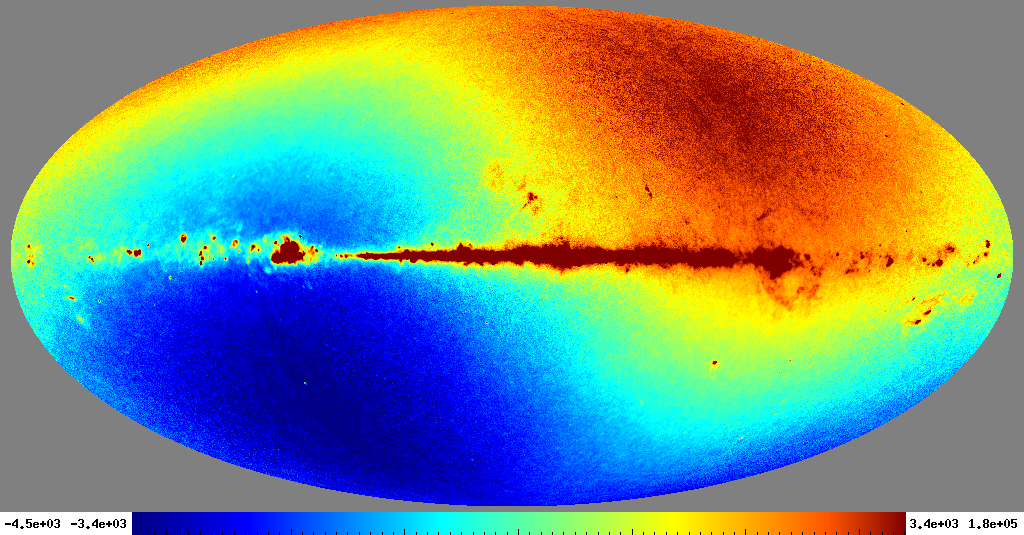
\includegraphics[width=0.49\textwidth]{figs/27M_map.png}
  \includegraphics[width=0.49\textwidth]{figs/27S_map.png}\\
  \includegraphics[width=0.49\textwidth]{figs/28M_map.png}
  \includegraphics[width=0.49\textwidth]{figs/28S_map.png}\\
  %\includegraphics[width=0.5\columnwidth]{figs/cbar_temp.pdf}\\
  \includegraphics[width=0.49\textwidth]{figs/Q_map.png}
  \includegraphics[width=0.49\textwidth]{figs/U_map.png}\\
  %\includegraphics[width=0.5\columnwidth]{figs/cbar_pol.pdf}\\
  \caption{Temperature and polarization maps of the LFI 30 GHz data produced using n+2 mapmaking. The top four panels contain the temperature maps, and the bottom row contains the combined Q and U maps.}
  \label{fig:maps}
\end{figure*}

\section{Bandpass correction}

Figure \ref{fig:bp_diffs} shows the 6 possible difference maps between the four temperature maps, smoothed to one degree to show their structure.

\begin{figure*}
\hspace{0.8in} 27S \hspace{2in} 28M \hspace{2in} 28S\\
  \centering
  27M \includegraphics[width=0.31\textwidth]{figs/tod_27M_minus_27S_map_c0001_k000001_1deg.png}
  \includegraphics[width=0.31\textwidth]{figs/tod_27M_minus_28M_map_c0001_k000001_1deg.png}
  \includegraphics[width=0.31\textwidth]{figs/tod_27M_minus_28S_map_c0001_k000001_1deg.png}\\
  \hspace{2.3in}
  27S \includegraphics[width=0.31\textwidth]{figs/tod_27S_minus_28M_map_c0001_k000001_1deg.png}
    \includegraphics[width=0.31\textwidth]{figs/tod_27S_minus_28S_map_c0001_k000001_1deg.png}\\
     \hspace{4.6in}
    28M \includegraphics[width=0.31\textwidth]{figs/tod_28M_minus_28S_map_c0001_k000001_1deg.png} \\
  %\includegraphics[width=0.5\columnwidth]{figs/cbar_pol.pdf}\\
  \caption{All 6 possible difference maps between the 30 Ghz detectors. }
  \label{fig:bp_diffs}
\end{figure*}

\begin{equation}
    \begin{aligned}
        d &= \textcolor{red}{U_{\text{ADC}} M_{\text{mod}} M_{\text{nlbol}}} \Bigg( \textcolor{red}{n_{4K} + n_{\text{bias}} + n_{\text{jump}} + n_{\text{dark}}} + n_{\text{corr}} + n_{\text{wn}} + \\
        &\quad \textcolor{red}{M_{\text{cross}}} \left[ G \textcolor{red}T P B \left\{ \int \tau(\nu; \Delta_{\text{bp}}) \big\{ s_{\text{sky}} + \textcolor{red}{s_{\text{zodi}}} + s_{\text{fsl}} + s_{\text{leak}} \big\} \, d\nu + s_{\text{orb}} \right\} + \textcolor{red}{n_{\text{CR}} + n_{\text{cross}}} \right] \Bigg)
    \end{aligned}
\end{equation}

\section{Conclusions and Future Plans}


\begin{acknowledgements}
 The current work has received funding from the European
  Union’s Horizon 2020 research and innovation programme under grant
  agreement numbers 819478 (ERC; \textsc{Cosmoglobe}) and 772253 (ERC;
  \textsc{bits2cosmology}). Some of the results in this paper have been derived using the HEALPix \citep{healpix} package.
  We acknowledge the use of the Legacy Archive for Microwave Background Data
  Analysis (LAMBDA), part of the High Energy Astrophysics Science Archive Center
  (HEASARC). HEASARC/LAMBDA is a service of the Astrophysics Science Division at
  the NASA Goddard Space Flight Center.  
  
   This publication makes use of data products from the Wide-field Infrared Survey Explorer, which is a joint project of the University of California, Los Angeles, and the Jet Propulsion Laboratory/California Institute of Technology, and NEOWISE, which is a project of the Jet Propulsion Laboratory/California Institute of Technology. WISE and NEOWISE are funded by the National Aeronautics and Space Administration.
   
   This work has made use of data from the European Space Agency (ESA) mission
{\it Gaia} (\url{https://www.cosmos.esa.int/gaia}), processed by the {\it Gaia}
Data Processing and Analysis Consortium (DPAC,
\url{https://www.cosmos.esa.int/web/gaia/dpac/consortium}). Funding for the DPAC
has been provided by national institutions, in particular the institutions
participating in the {\it Gaia} Multilateral Agreement.
\end{acknowledgements}


%-------------------------------------------------------------
%                                       Table with references 
%-------------------------------------------------------------
%

\bibliographystyle{aa}
\bibliography{references, ../../common/CG_bibliography}
\end{document}
%%%% End of aa.dem
